% Drawing 146/04-2 -- folder 146, batch 04, archive page 61 (PDF page 62).
% Transcription: Dans la colonne de gauche, trois sphères : la première porte un cercle équatorial avec cinq points marqués ; la deuxième un sommet au pôle relié par des arcs à quatre points de l'équateur ; la troisième des cercles méridiens et un axe pointillé, avec des points marqués aux pôles et sur l'équateur.
% Kind: cell decompositions of the sphere. Method 3 (encoded, rendered from the data). Status: ok.
% Notes: Three spheres. 1: equator with five ringed points. 2: a ringed pole joined by four arcs (one dashed, behind) to four ringed points of the equator. 3: meridian circles, dotted polar axis, ringed points at both poles, at the centre and at both ends of the equator -- redrawn but not encoded (the number of meridians is not certain: two are clearly drawn). He gives no counts here, so the encodings are checked only for Euler (chi = 2). Text in the left margin (Z/5Z, D5 ...) belongs to the transcription.
% Coordinates: 1 unit = 1 mm = 1/100 of the crop width (bbox in page fractions: [0.26, 0.225, 0.49, 0.62]).
% Redrawn by Claude (claude-opus-5-5), issue #73 pilot, 2026-11-07; not checked by a human; not compiled (no TeX in the session).
% Rights: reproduces part of the work -- behind RENDER_TRANSCRIPTS, never published by itself.
\documentclass[tikz,border=3pt]{standalone}
\usepackage{amsmath,amssymb}
\usetikzlibrary{patterns,arrows.meta}
\tikzset{pencil/.style={black!45}, struck/.style={black!35}, mark/.style={circle,draw,inner sep=1.3pt}, pt/.style={circle,fill,inner sep=0.9pt}, opt/.style={circle,draw,fill=white,inner sep=1.1pt}}
\begin{document}
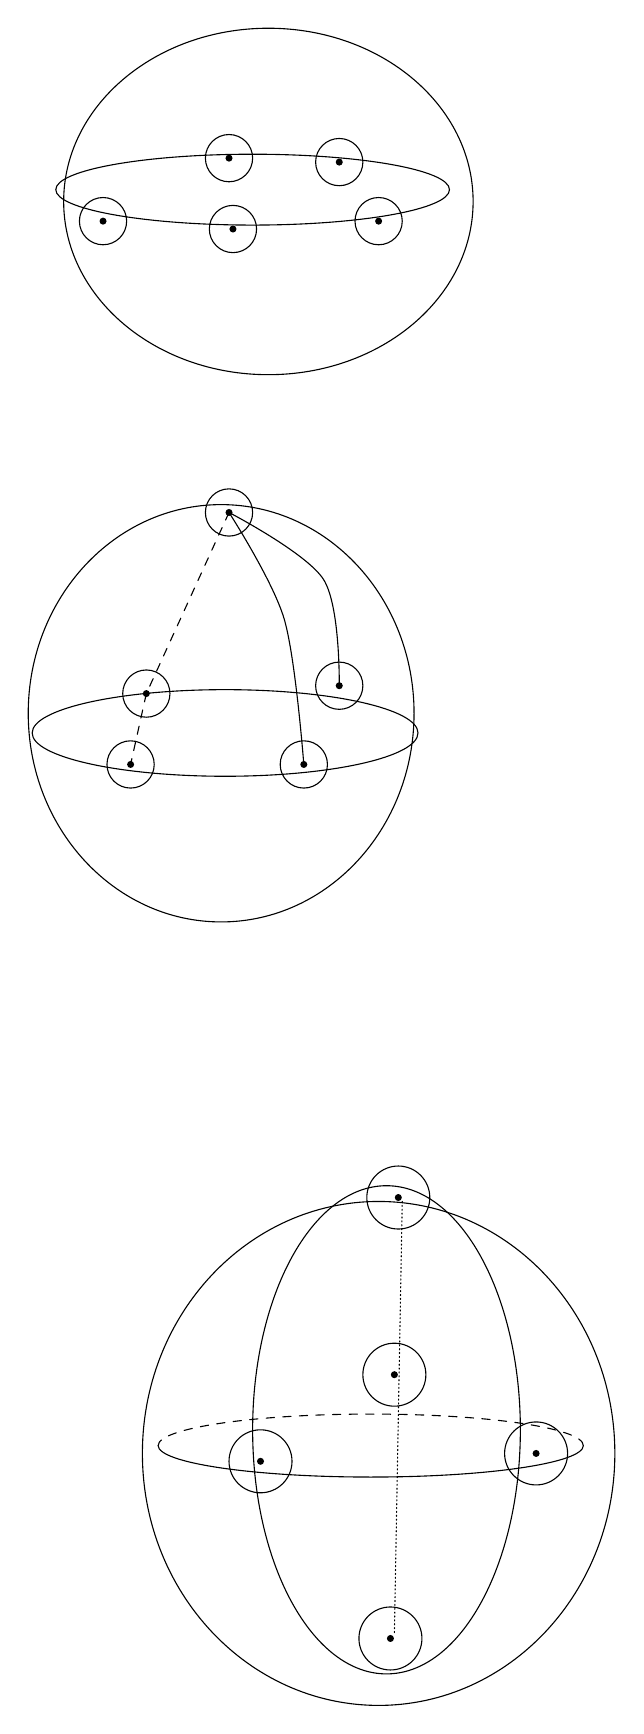
\begin{tikzpicture}[x=1mm,y=1mm,line cap=round,line join=round,font=\scriptsize]
\draw (43,-26.2) ellipse[x radius=26, y radius=22];
\draw (66,-24.7) arc[start angle=0, end angle=180, x radius=25, y radius=4.5];
\draw (16,-24.7) arc[start angle=180, end angle=360, x radius=25, y radius=4.5];
\draw (38,-20.7) circle[radius=3];
\draw (52,-21.2) circle[radius=3];
\draw (22,-28.7) circle[radius=3];
\draw (38.5,-29.7) circle[radius=3];
\draw (57,-28.7) circle[radius=3];
\node[pt] at (38,-20.7) {};
\node[pt] at (52,-21.2) {};
\node[pt] at (22,-28.7) {};
\node[pt] at (38.5,-29.7) {};
\node[pt] at (57,-28.7) {};
\draw (37,-91.2) ellipse[x radius=24.5, y radius=26.5];
\draw (37.5,-93.7) ellipse[x radius=24.5, y radius=5.5];
\draw[dashed] (38,-65.7) -- (27.5,-88.7) -- (25.5,-97.7);
\draw plot[smooth, tension=0.55] coordinates {(38,-65.7) (45,-79.2) (47.5,-97.7)};
\draw plot[smooth, tension=0.55] coordinates {(38,-65.7) (50,-74.2) (52,-87.7)};
\draw (38,-65.7) circle[radius=3];
\draw (27.5,-88.7) circle[radius=3];
\draw (52,-87.7) circle[radius=3];
\draw (25.5,-97.7) circle[radius=3];
\draw (47.5,-97.7) circle[radius=3];
\node[pt] at (38,-65.7) {};
\node[pt] at (27.5,-88.7) {};
\node[pt] at (52,-87.7) {};
\node[pt] at (25.5,-97.7) {};
\node[pt] at (47.5,-97.7) {};
\draw (57,-185.2) ellipse[x radius=30, y radius=32];
\draw (58,-182.2) ellipse[x radius=17, y radius=31];
\draw[dashed] (83,-184.2) arc[start angle=0, end angle=180, x radius=27, y radius=4];
\draw (29,-184.2) arc[start angle=180, end angle=360, x radius=27, y radius=4];
\draw[densely dotted] (60,-153.2) -- (59,-208.2);
\draw (59.5,-152.7) circle[radius=4];
\draw (58.5,-208.7) circle[radius=4];
\draw (59,-175.2) circle[radius=4];
\draw (42,-186.2) circle[radius=4];
\draw (77,-185.2) circle[radius=4];
\node[pt] at (59.5,-152.7) {};
\node[pt] at (58.5,-208.7) {};
\node[pt] at (59,-175.2) {};
\node[pt] at (42,-186.2) {};
\node[pt] at (77,-185.2) {};
\end{tikzpicture}
\end{document}
